\chapter{Ripasso di programmazione II}

In questa sezione si andranno a ripassare e approfondire alcuni argomenti del corso di programmazione II come:

\begin{itemize}
    \item L'ereditarietà;
    \item Estensioni di classi;
    \item Polimorfismo;
    \item Downcasting e upcasting;
    \item Overriding;
    \item Classi astratte;
    \item Interfacce.
\end{itemize}

\section{L'ereditarietà}

\dfn{Ereditarietà}{L'\textbf{ereditarietà} è un meccanismo della programmazione a oggetti che consente di espandere alcune classi aggiungendo attributi e/o metodi.}

\cor{Sottoclassi}{Le \textbf{sottoclassi} ereditano tutti i componenti della propria sovraclasse (variabili e metodi). }

\begin{figure}[h]
\caption{Esempio di ereditarietà}
\begin{center}
    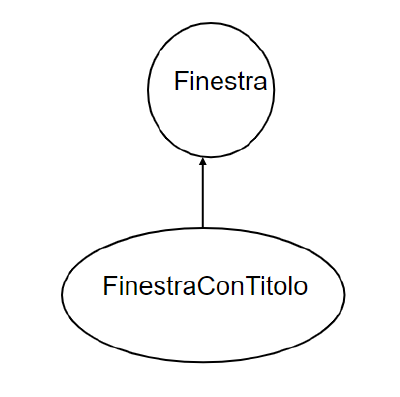
\includegraphics[scale=0.5]{images/ripasso di programmazione II/Finestra.png}
\end{center}
\end{figure}

\nt{In Java l'ereditarietà è singola, per cui ogni classe ha un solo genitore\footnote{E ogni classe discende dalla classe Object}.}

\section{Tipi e metodi}

\dfn{Controllo dei tipi}{Java effettua un controllo statico per i tipi (prima dell'esecuzione). Il \textbf{checking} controlla che per una variabile si  chiami un metodo definito per la classe di quella variabile. }

\dfn{Polimorfismo}{Un oggetto può avere \underline{più} di un tipo. Per esempio un oggetto di tipo E che è figlio di un oggetto di tipo C ha entrambi i tipi (E e C). Dato il tipo di una varabile x (A) e un espressione di tipo (B), x = expr è legale se e solo se A = B oppure se B è una sottoclasse di A.}

\cor{Upcasting e downcasting}{L'\textbf{upcasting} è un movimento da un tipo specifico a uno più generico. Questo assegnamento è sempre legale, per esempio, tutti i cani (specifico) sono animali (generico) oppure tutti i rettangoli (specifico) sono poligoni (generico). Se si effettua un upcasting non si possono più utilizzare i metodi della sottoclasse.

Il \textbf{downcasting} è l'operazione opposta.}

\cor{Overriding}{L'\textbf{overriding} permette a una sottoclasse di sovrascrivere un metodo di una sovraclasse. Per fare ciò si scrive nella sottoclasse un metodo con una firma  uguale a un metodo della sovraclasse e si cambia il corpo. Un classico esempio è la funzione toString.}

\nt{Di default toString restituisce il nome della classe + @ + codici alfanumerici}

\cor{Super}{Si può usare il codice della classe genitore nella classe figlio mediante la classe \textbf{super}. Normalmente se si vuole utilizzare super lo si deve fare come prima cosa. Se non esiste una classe super nel genitore si può causare un loop infinito.}

\dfn{Visibilità}{
\begin{itemize}
    \item \textbf{private}: si vede solo all'interno della classe;
    \item \textbf{protected}: visibile da classi e sottoclassi nello stesso package;
    \item \textbf{public}: visibile da tutti.
\end{itemize}
}

\dfn{Binding dinamico}{Nel \textbf{binding dinamico} si crea un legame durante l'esecuzione. Questo avviene in quasi tutti i linguaggi a oggetti (eccezione C++). In C++ si deve ricorrere all'upcasting. In java non è presente il binding dinamico con le variabili.}

\section{Programmare con l'ereditarietà}

Per ricapitolare, i linguaggi a oggetti:

\begin{itemize}
    \item hanno una struttura modulare;
    \item implementano tipi di dati astratti;
    \item offrono gestione automatica della memoria (garbage collector);
    \item hanno classi;
    \item ereditarietà singola o multipla;
    \item polimorfismo e binding dinamico.
\end{itemize}

\dfn{Riuso del software}{Il programmare a oggetti rende possibile riusare il software:

\begin{itemize}
    \item con il \textbf{contenimento} si definiscono nuove classi i cui oggetti sono già compresi in altre classi. Per esempio l'\textbf{automobile} ha un \textbf{motore}, ha delle \textbf{ruote}, etc.;
    \item con l'\textbf{ereditarietà} si estendono delle classi già esistenti. Per esempio un \textbf{poligono} può essere un \textbf{triangolo}, un \textbf{parallelogramma}, etc. 
\end{itemize}
}

\dfn{Classi astratte}{Alcuni classi possono essere \textbf{astratte} per cui non è necessario implementare il codice di un metodo in cui si specifica solo la firma. Questi metodi estratti servono da interfaccie di metodi usati dalle sottoclassi. Le classi astratte hanno un \textbf{costruttore}, ma non possono essere istanziate.
}

\dfn{Interfacce}{Le \textbf{interfacce} sono strutture simili a delle classi, ma possono contenere solo metodi astratti.}

\nt{Un programma può implementare più di un'interfaccia.}

\subsection{Reflection}

\dfn{Reflection}{La reflection consiste nell'interrogare un oggetto per accertarne alcune caratteristiche.}

\cor{instanceof}{
Per essere sicuri che la classe di un oggetto, a runtime, sia corretta si usa la instanceof. instanceof restituisce true se l'oggetto è istanza di un certa classe, false altrimenti.
}

\nt{instanceof è un particolare tipo di reflection.}

\dfn{La classe Class}{
In java la classe Class contiene tutte le classi C usate in un programma. Rappresenta il \textit{tipo} di un oggetto.
}

\cor{isInstance}{
isInstance è un metodo di Class che funziona come una versione dinamica di instanceof.
}

\cor{getClass}{getClass è un metodo che restutuisce la classe dell'oggetto su cui è invocato.}

\cor{getName}{getName è un metodo che restutuisce, come stringa, il nome dell'oggetto su cui è invocato.}

\cor{forName}{forName è un metodo che carica una classe.}

\cor{getSuperclass}{getSuperclass è un metodo che restutuisce la sopraclasse dell'oggetto su cui è invocato.}

\cor{newInstance}{newInstance è un metodo che crea un nuovo oggetto con la stessa classe dell'oggetto su cui è invocato.}

\nt{newInstance non viene mai usato, perchè si preferisce usare "new"}.

\dfn{java.lang.reflect}{
Il package java.lang.reflect contiene le classi Field, Methods e Constructor.

\paragraph{Class contiene:}
\begin{itemize}
    \item getFields: restituisce un array con i campi della classe su cui è invocato;
    \item getMethods: restituisce un array con i metodi della classe su cui è invocato;
    \item getConstructor: restituisce un array con i costruttori della classe su cui è invocato.
\end{itemize}

\paragraph{Methods contiene:}
\begin{itemize}
    \item getParameterTypes;
    \item invoke.
\end{itemize}

}

\section{Trattamento delle eccezioni}

Durante l'esecuzione di un programma possono verificarsi degli errori.

\begin{itemize}
    \item errori di programmazione;
    \item dati errati in ingresso.
\end{itemize}

\nt{Ci vuole una separazione tra la gestione degli errori e i risultati dei metodi.}

\dfn{Le eccezioni}{Il meccanismo delle eccezioni serve per gestire gli errori veri e propri e anche i casi straordinari.}

\cor{Soluzione banale}{
La prima soluzione che si impara è quella di restituire un valore riservato che indica il successo o il fallimento.
}

\nt{Tuttavia non sempre questo è possibile.}

\dfn{Throw, try e catch}{
Il costrutto throw serve per lanciare le eccezioni. Il costrutto try serve per eseguire istruzioni che potrebbero lanciare eccezioni e catturarle con il costrutto catch (exception handler).
}

\nt{Le eccezioni hanno un determinato tipo (sono oggetti throwable\footnote{Errori irreparabili o eccezioni}). Inoltre gli errori hanno un campo message che specifica il perchè l'errore è avvenuto.}

\dfn{Finally}{Il costrutto finally è sempre eseguito (anche se non sono sollevate eccezioni).}

\ex{Chiusura di un file}{
Le modifiche a un file non sono permanenti finchè non si chiude. In questo caso è utile utilizzare il costrutto finally per chiudere il file sia nel caso in cui non si siano verificate eccezioni sia nel caso ne siano state sollevate.
}

\dfn{Definizione di eccezioni}{Si possono definire eccezioni personalizzate che andranno a estendere Exception o RuntimeException.}

\nt{
\paragraph{Alcuni suggerimenti:}
\begin{itemize}
    \item le eccezioni non devono essere gestite in modo troppo frammentario;
    \item mettere i catch più specifici per primi e i più generici per ultimi;
    \item non si devono silenziare le eccezioni;
    \item se si cattura un errore è preferibile essere severi;
    \item a volte conviene passare un'eccezione invece di gestirla subito.
\end{itemize}
}

\section{Gestione della memoria}

\dfn{Compilazione}{
La compilazione dei programmi scritti in Java prende in input il codice sorgente e restituisce in output il byte code (eseguibile su differenti S.O.).
}

\begin{figure}[ht]
\caption{Come viene compilato un programma Java}
\begin{center}
    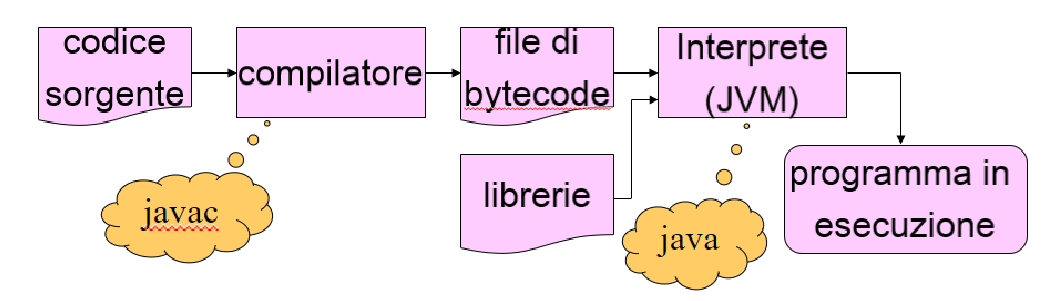
\includegraphics[scale=0.3]{images/ripasso di programmazione II/Compilazione.png}
\end{center}
\end{figure}

\nt{Alcuni IDE, come IntelliJ, automatizzano questo processo.}

\dfn{Memoria della JVM}{
La memoria della JVM è organizzata in:
\begin{itemize}
    \item [$\Rightarrow$] memoria statica: mantiene tutte le parti statiche del programma (alcune variabili, costanti, il codice delle clssi, etc.);
    \item [$\Rightarrow$] stack: è gestito come una pila LIFO (Last In First Out), mantiene i record di attivazioni;
    \item [$\Rightarrow$] heap: presenta il garbage collector e mantiene i dati creati dinamicamente.
\end{itemize}
}

\nt{I metodi che non hanno bisogno di accedere allo stato di un oggetto vanno dichiarati static}

\dfn{Record di attivazione (frame)}{
I record di attivazione contengono i dati necessari a gestire l'esecuzione di un metodo. Contengono:
\begin{itemize}
    \item parametri formali;
    \item varabili locali;
    \item risultato di ritorno (per metodi non-void);
    \item l'indirizzo di ritorno.
\end{itemize}
}

\dfn{Variabili statiche e di istanza}{
\paragraph{Variabili statiche:} c'è una sola copia di queste variabili ed è condivisa fra tutti gli oggetti di una determinata classe.
\paragraph{Variabili di istanza (o dinamiche):} memorizzano lo stato degli oggetti. Ogni oggetto ne ha una copia nel heap.
}